\documentclass[journal,12pt,twocolumn]{IEEEtran}

\usepackage{setspace}
\usepackage{gensymb}

\singlespacing


\usepackage[cmex10]{amsmath}

\usepackage{amsthm}

\usepackage{mathrsfs}
\usepackage{txfonts}
\usepackage{stfloats}
\usepackage{bm}
\usepackage{cite}
\usepackage{cases}
\usepackage{subfig}

\usepackage{longtable}
\usepackage{multirow}

\usepackage{enumitem}
\usepackage{mathtools}
\usepackage{steinmetz}
\usepackage{tikz}
\usepackage{circuitikz}
\usepackage{verbatim}
\usepackage{tfrupee}
\usepackage[breaklinks=true]{hyperref}
\usepackage{graphicx}
\usepackage{graphics}
\usepackage{tkz-euclide}
\usepackage{float}

\usetikzlibrary{calc,math}
\usepackage{listings}
    \usepackage{color}                                            %%
    \usepackage{array}                                            %%
    \usepackage{longtable}                                        %%
    \usepackage{calc}                                             %%
    \usepackage{multirow}                                         %%
    \usepackage{hhline}                                           %%
    \usepackage{ifthen}                                           %%
    \usepackage{lscape}     
\usepackage{multicol}
\usepackage{chngcntr}

\DeclareMathOperator*{\Res}{Res}

\renewcommand\thesection{\arabic{section}}
\renewcommand\thesubsection{\thesection.\arabic{subsection}}
\renewcommand\thesubsubsection{\thesubsection.\arabic{subsubsection}}

\renewcommand\thesectiondis{\arabic{section}}
\renewcommand\thesubsectiondis{\thesectiondis.\arabic{subsection}}
\renewcommand\thesubsubsectiondis{\thesubsectiondis.\arabic{subsubsection}}


\hyphenation{op-tical net-works semi-conduc-tor}
\def\inputGnumericTable{}                                 %%

\lstset{
%language=C,
frame=single, 
breaklines=true,
columns=fullflexible
}
\begin{document}


\newtheorem{theorem}{Theorem}[section]
\newtheorem{problem}{Problem}
\newtheorem{proposition}{Proposition}[section]
\newtheorem{lemma}{Lemma}[section]
\newtheorem{corollary}[theorem]{Corollary}
\newtheorem{example}{Example}[section]
\newtheorem{definition}[problem]{Definition}

\newcommand{\BEQA}{\begin{eqnarray}}
\newcommand{\EEQA}{\end{eqnarray}}
\newcommand{\define}{\stackrel{\triangle}{=}}
\newcommand\hlight[1]{\tikz[overlay, remember picture,baseline=-\the\dimexpr\fontdimen22\textfont2\relax]\node[rectangle,fill=blue!50,rounded corners,fill opacity = 0.2,draw,thick,text opacity =1] {$#1$};}
\bibliographystyle{IEEEtran}
\providecommand{\mbf}{\mathbf}
\providecommand{\pr}[1]{\ensuremath{\Pr\left(#1\right)}}
\providecommand{\qfunc}[1]{\ensuremath{Q\left(#1\right)}}
\providecommand{\sbrak}[1]{\ensuremath{{}\left[#1\right]}}
\providecommand{\lsbrak}[1]{\ensuremath{{}\left[#1\right.}}
\providecommand{\rsbrak}[1]{\ensuremath{{}\left.#1\right]}}
\providecommand{\brak}[1]{\ensuremath{\left(#1\right)}}
\providecommand{\lbrak}[1]{\ensuremath{\left(#1\right.}}
\providecommand{\rbrak}[1]{\ensuremath{\left.#1\right)}}
\providecommand{\cbrak}[1]{\ensuremath{\left\{#1\right\}}}
\providecommand{\lcbrak}[1]{\ensuremath{\left\{#1\right.}}
\providecommand{\rcbrak}[1]{\ensuremath{\left.#1\right\}}}
\theoremstyle{remark}
\newtheorem{rem}{Remark}
\newcommand{\sgn}{\mathop{\mathrm{sgn}}}
\providecommand{\abs}[1]{\left\vert#1\right\vert}
\providecommand{\res}[1]{\Res\displaylimits_{#1}} 
\providecommand{\norm}[1]{\left\lVert#1\right\rVert}
%\providecommand{\norm}[1]{\lVert#1\rVert}
\providecommand{\mtx}[1]{\mathbf{#1}}
\providecommand{\mean}[1]{E\left[ #1 \right]}
\providecommand{\fourier}{\overset{\mathcal{F}}{ \rightleftharpoons}}
%\providecommand{\hilbert}{\overset{\mathcal{H}}{ \rightleftharpoons}}
\providecommand{\system}{\overset{\mathcal{H}}{ \longleftrightarrow}}
	%\newcommand{\solution}[2]{\textbf{Solution:}{#1}}
\newcommand{\solution}{\noindent \textbf{Solution: }}
\newcommand{\cosec}{\,\text{cosec}\,}
\providecommand{\dec}[2]{\ensuremath{\overset{#1}{\underset{#2}{\gtrless}}}}
\newcommand{\myvec}[1]{\ensuremath{\begin{pmatrix}#1\end{pmatrix}}}
\newcommand{\mydet}[1]{\ensuremath{\begin{vmatrix}#1\end{vmatrix}}}
\numberwithin{equation}{subsection}
\makeatletter
\@addtoreset{figure}{problem}
\makeatother
\let\StandardTheFigure\thefigure
\let\vec\mathbf
\renewcommand{\thefigure}{\theproblem}
\def\putbox#1#2#3{\makebox[0in][l]{\makebox[#1][l]{}\raisebox{\baselineskip}[0in][0in]{\raisebox{#2}[0in][0in]{#3}}}}
     \def\rightbox#1{\makebox[0in][r]{#1}}
     \def\centbox#1{\makebox[0in]{#1}}
     \def\topbox#1{\raisebox{-\baselineskip}[0in][0in]{#1}}
     \def\midbox#1{\raisebox{-0.5\baselineskip}[0in][0in]{#1}}
\vspace{3cm}
\title{Assignment 10}
\author{SOWMYA BANDI}
\maketitle
\newpage
\bigskip
\renewcommand{\thefigure}{\theenumi}
\renewcommand{\thetable}{\theenumi}
Download all python codes from 
\begin{lstlisting}
https://github.com/Sowmyabandi99/Assignment10/blob/main/assignment10_2.py
\end{lstlisting}
%
and latex-tikz codes from 
%
\begin{lstlisting}
https://github.com/Sowmyabandi99/Assignment10/blob/main/main.tex
\end{lstlisting}
%
\section{Question No. 2.26}
A manufacturer makes two types of toys A and B. Three machines are needed for this purpose and the time (in minutes) required for each toy on the machines is given below: \\
\numberwithin{table}{section}
\begin{table}[!ht]
\begin{center}
\begin{tabular}{|l|l|l|l|} \hline
\multicolumn{4}{|c|} {Machines} \\ \hline
Types of toys & I & II & III \\ \hline
A & 12 & 18 & 6\\ \hline
B & 6 & 0 & 9\\ \hline
\end{tabular}
\end{center}
\caption{Toys table}
\label{opt/26/tab:table1}
\end{table}\\
Each machine is available for a maximum of 6 hours per day. If the profit on each toy of type A is Rs 7.50 and that on each toy of type B is Rs 5, show that 15 toys of type A and 30 of type B should be manufactured in a day to get maximum profit.
%
\section{Solution}
Let the number of toys of type A be $x$ and the number of toys of type B be $y$  such that 
\begin{align}
    x \geq 0 \\
    y \geq 0 
\end{align}
According to the question,
\begin{align}
    12x+6y &\leq 360 \\
    \implies 2x+y &\leq 60 
\end{align}
and,
\begin{align}
    18x+0y &\leq 360 \\
    \implies x &\leq 20
\end{align}
and,
\begin{align}
     6x+9y &\leq 360 \\
    \implies 2x+3y &\leq 120 
\end{align}
$\therefore$ Our problem is
\begin{align}
        \max_{\vec{x}} Z &= \myvec{7.5 & 5}\vec{x}\\
        s.t. \quad 
        \myvec{2 & 1 \\ 1 & 0 \\2 & 3 }\vec{x} &\preceq \myvec{60\\20\\120} 
\end{align}
Lagrangian function is given by
\begin{equation}
\begin{aligned}
    &L(\vec{x},\boldsymbol{\lambda}) \\ &= \myvec{7.5 & 5}\vec{x}+\lcbrak{\sbrak{\myvec{2 & 1}\vec{x}-60}} \\ &+ \sbrak{\myvec{1 & 0}\vec{x}-20} +\sbrak{\myvec{2 & 3}\vec{x}-120} \\ &+ \sbrak{\myvec{-1 & 0}\vec{x}} +\rcbrak{\sbrak{\myvec{0 & -1}\vec{x}}}\boldsymbol{\lambda}
\end{aligned}
\end{equation}
where,
\begin{align}
    \boldsymbol{\lambda} &= \myvec{\lambda_1 \\ \lambda_2 \\ \lambda_3 \\ \lambda_4 \\ \lambda_5 \\ \lambda_6}
\end{align}
Now,
\begin{align}
    \nabla L(\vec{x},\boldsymbol{\lambda}) &= \myvec{7.5+ \myvec{2 & 1 & 2 & -1 & 0 }\boldsymbol{\lambda}\\ 5+\myvec{1 & 0 & 3 & 0 & -1}\boldsymbol{\lambda} \\ \myvec{2 & 1}\vec{x}-60 \\ \myvec{1 & 0}\vec{x}-20 \\ \myvec{2 & 3}\vec{x}-120 \\ \myvec{-1 & 0}\vec{x} \\ \myvec{0 & -1}\vec{x}}
\end{align}
$\therefore$ Lagrangian matrix is given by
\begin{align}
    \myvec{0 & 0 & 2 & 1 & 2 & -1 & 0 \\ 0 & 0 & 1 & 0 & 3 & 0 & -1 \\ 2 & 1 & 0 & 0 & 0 & 0 & 0 \\ 1 & 0 & 0 & 0 & 0 & 0 & 0 \\ 2 & 3 & 0 & 0 & 0 & 0 & 0 \\ -1 & 0 & 0 & 0 & 0 & 0 & 0 \\ 0 & -1 & 0 & 0 & 0 & 0 & 0 }\myvec{\vec{x} \\ \boldsymbol{\lambda} } &= \myvec{-7.5 \\ -5 \\ 60 \\ 20 \\ 120 \\ 0 \\0 }
\end{align}
Considering $\lambda_1,\lambda_2$ as only active multiplier,
\begin{align}
    \myvec{0 & 0 & 2 & 2 \\ 0 & 0 & 1 & 3 \\ 2 & 1 & 0 & 0 \\ 2 & 3 & 0 & 0}\myvec{\vec{x}\\ \boldsymbol{\lambda}} &= \myvec{-7.5 \\ -5 \\ 60 \\ 120}
\end{align}
resulting in,
\begin{align}
    \myvec{\vec{x} \\ \boldsymbol{\lambda}} &= \myvec{0 & 0 & 2 & 2 \\ 0 & 0 & 1 & 3 \\ 2 & 1 & 0 & 0 \\ 2 & 3 & 0 & 0}^{-1}\myvec{-7.5 \\ -5 \\ 60 \\ 120}
    \\
    \implies   \myvec{\vec{x} \\ \boldsymbol{\lambda}} &= \myvec{0 & 0 & \frac{3}{4} & \frac{-1}{4} \\ 0 & 0 & \frac{-1}{2} & \frac{1}{2} \\ \frac{3}{4} & \frac{-1}{2} & 0 & 0 \\ \frac{1}{4} & \frac{1}{2} & 0 & 0}\myvec{-7.5 \\ -5 \\ 60 \\ 120}
    \\
    \implies \myvec{\vec{x} \\ \boldsymbol{\lambda}} &= \myvec{15 \\ 30 \\ -3.12 \\ -0.62}
\end{align}
$\because \boldsymbol{\lambda}=\myvec{-3.12 \\ -0.62} \succ \vec{0} $
\\
$\therefore$ Optimal solution is given by
\begin{align}
    \vec{x} &= \myvec{15\\30} \\
    Z &= \myvec{7.5 & 5}\vec{x} \\
    &= \myvec{7.4 & 5}\myvec{15 \\ 30} \\
    &= 262.5
\end{align}
By using cvxpy in python ,
\begin{align}
    \vec{x}=\myvec{14.99999998\\29.99999996}\\
    Z = 262.49999967
\end{align}
Hence, the manufacturer should manufacture \boxed{x=15} toys of type A and \boxed{y=30} toys of type B in a day to get maximum profit \boxed{Z=262.5}.
\numberwithin{figure}{section}
\begin{figure}[!ht]
\centering
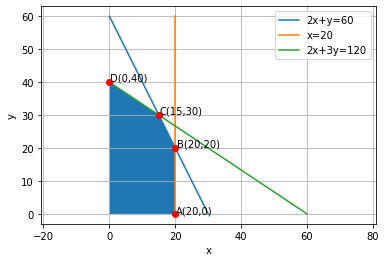
\includegraphics[width=\columnwidth]{Figure10}
\caption{Diet Problem}
\label{fig:toy problem}	
\end{figure}
\end{document}
29.99999996